%%
% Template for using the IEEEtran documentclass
% Uses onecolumn journal style with 10 pt font
%%
\documentclass[journal,onecolumn,twoside,10pt]{IEEEtran}

%% Include any other packages you want here.
\usepackage{lipsum} % Generate dummy text.
\usepackage{graphicx} % Enable graphics

% "Double" spacing
\linespread{1.6}

% paper title
% can use linebreaks \\ within to get better formatting as desired
\title{Sample Document for CprE 308}

% Author Name
\author{Your~Name} 

%% Header info.  First part for page one and even, second for odd after first.
\markboth{CPRE 308 FINAL PROJECT, SPRING 2014}
{LAST~NAME: TITLE}

% Begin document
\begin{document}

% Include title information
\maketitle

% Use the input command to include other files (notice we don't need the extension)
% Feel free to add as many files as necessary.

\begin{abstract}
The abstract goes here.
\end{abstract}

\section{Introduction}
\label{s:intro} % This declares a label so you can reference the section elsewhere.

\IEEEPARstart{T}{his} is a template intended to assist students writing their final reports.
Notice the command at the start of this paragraph - it is optional but adds a nice effect to the report.
If you have any questions, feel free to contact me and let me know.
Otherwise you can simply fill in this template with your text.
That's it for text.  Lorem Ipsum from here on.

\subsection{Subsection heading}
\lipsum[1] % Generate one paragraph of lipsum

\subsection{This is another heading}
\lipsum[2-3]

\subsection{Summary}
% To reference other labels, simply use \ref{}
% ~ is a space, but forces the surrounding words to remain on the same line.
The remainder of the paper is organized as follows:
Section~\ref{s:background} will discuss background information.
In Section~\ref{s:topic} we discuss our main topic.
Finally, we conclude in Section~\ref{s:conclusion}

\section{Background}
\label{s:background} % This declares a label so you can reference the section elsewhere.

Background material can go here.
(Or whatever other content you want).

Follows is an example of a reference.
The authors of~\cite{Humar2011} conclude interesting things.

\subsection{Subtopic 1}
\lipsum[4]

\subsection{Subtopic 2}
\lipsum[5]

\section{Topic}
\label{s:topic} % This declares a label so you can reference the section elsewhere.

Talk about your main points here.
Perhaps add additional sections as necessary to break it into logical sections.
Good stuff.

\subsection{Information}

This is a bulleted list:
\begin{itemize}
\item Item 1
\item Item 2
\item Item 3
\item Item 4
\end{itemize}

This is a numbered list:
\begin{enumerate}
\item Item 1
\item Item 2
\item Item 3
\item Item 4
\end{enumerate}

\subsection{How to make a figure}
Sometimes you want figures in your paper.
Use the includegraphics command to insert figures, like in Figure~\ref{f:os_block}.

\begin{figure}
\centering % Make it center
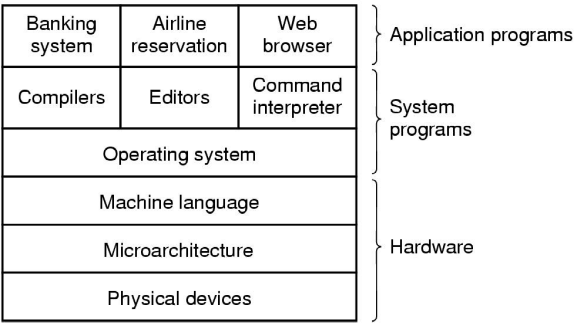
\includegraphics[width=0.5\textwidth]{figures/os_block.png}
\caption{This is a caption for the figure}
\label{f:os_block}
\end{figure}

\subsection{How to include a table}
Tables are created using the tabular environment.
You can see it in Table~\ref{t:my_table}.

\begin{table}
\centering % Make it center
\begin{tabular}{l|cc} % Second argument is column list, one character per.  Justify with lcr.  Pipe for horizontal line
Name & Col 1 & Col 2 \\ % Separate columns with &, end line with \\
\hline % Horizontal line
Item 1 & 1 & 2 \\
Item 2 & 3 & 4\\
\end{tabular}
\caption{This is a caption for the table}
\label{t:my_table}
\end{table}

\subsection{More Fake Text}
More fake text here, but in subsections.

\subsubsection{Fizz}
\lipsum[6-8]

\subsubsection{Buzz}
\lipsum[9-10]

\section{Conclusion}
\label{s:conclusion} % This declares a label so you can reference the section elsewhere.

Conclude your report here.

\lipsum[11-12]


%% Include the bibliogrhy, using the IEEEtran style.
\bibliographystyle{IEEEtran}
\bibliography{reference} % Use bib information from reference.bib

% that's all folks
\end{document}


